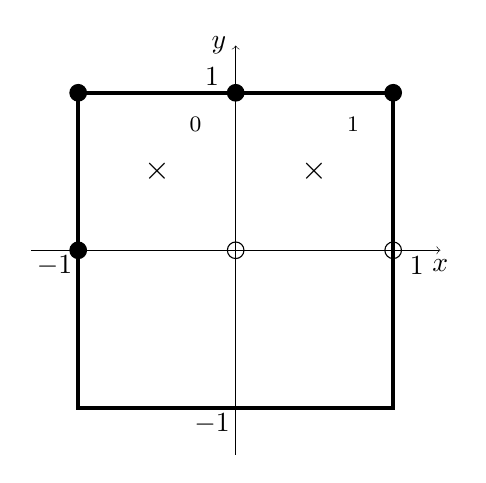
\begin{tikzpicture}[scale=2.0]
% origin of axes at (0.0,0.0) and square has half-width 1.0
  \draw[->,very thin] (-1.3,0.0) -- (1.3,0.0) node[below] {$x$};
  \draw[->,very thin] (0.0,-1.3) -- (0.0,1.3) node[left] {$y$};
  \draw[line width=1.5pt] (-1,-1) -- (1,-1) -- (1,1) -- (-1,1) -- cycle;
  \node at (1.15,-0.1) {$1$};
  \node at (-1.15,-0.1) {$-1$};
  \node at (-0.15,1.1) {$1$};
  \node at (-0.15,-1.1) {$-1$};
  \node at (-0.25,0.8) {\large $\square_0$};
  \node at (0.75,0.8) {\large $\square_1$};
  \draw (0.0,0.0) circle (1.5pt);
  \draw (1.0,0.0) circle (1.5pt);
  \filldraw (-1.0,0.0) circle (1.5pt);
  \filldraw (-1.0,1.0) circle (1.5pt);
  \filldraw (0.0,1.0) circle (1.5pt);
  \filldraw (1.0,1.0) circle (1.5pt);
  \node at (-0.5,0.5) {\large $\times$};
  \node at (0.5,0.5) {\large $\times$};
  %\filldraw (0.5,0.5) circle (1.0pt) node[xshift=6mm,yshift=2mm] {$foo$};
\end{tikzpicture}

